\documentclass[border=2pt]{standalone}
\usepackage{amssymb,amsmath}
\usepackage{tikz-cd}
\usepackage{physics}
\usetikzlibrary{arrows}

\usepackage{tikz}
\let\OX\bigotimes
\newcommand{\OP}{\displaystyle\bigoplus}
\let\ox\otimes
\let\op\oplus
\let\isom\cong
\let\vf\varphi
\begin{document}


\tikzset{every picture/.style={line width=0.75pt}} %set default line width to 0.75pt        

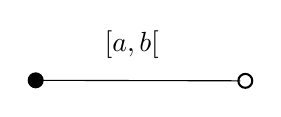
\begin{tikzpicture}[x=0.75pt,y=0.75pt,yscale=-1,xscale=1]
%uncomment if require: \path (0,300); %set diagram left start at 0, and has height of 300

%Straight Lines [id:da04388130101621468] 
\draw    (100,100) -- (198.65,100.24) ;
\draw [shift={(201,100.25)}, rotate = 0.14] [color={rgb, 255:red, 0; green, 0; blue, 0 }  ][line width=0.75]      (0, 0) circle [x radius= 3.35, y radius= 3.35]   ;
\draw [shift={(100,100)}, rotate = 0.14] [color={rgb, 255:red, 0; green, 0; blue, 0 }  ][fill={rgb, 255:red, 0; green, 0; blue, 0 }  ][line width=0.75]      (0, 0) circle [x radius= 3.35, y radius= 3.35]   ;


% Text Node
\draw (132,74.9) node [anchor=north west][inner sep=0.75pt]    {$[ a,b[$};

\end{tikzpicture}

\end{document}